\documentclass[11pt]{article}

\usepackage[margin=1in]{geometry}
\usepackage[T1]{fontenc}
\usepackage{lmodern}
\usepackage{microtype}
\usepackage{hyperref}
\usepackage{xcolor}
\usepackage{enumitem}
\usepackage{booktabs}
\usepackage{longtable}
\usepackage{listings}
\usepackage{tikz}
\usetikzlibrary{arrows.meta,positioning,shapes.geometric}

\hypersetup{
  colorlinks=true,
  linkcolor=blue!55!black,
  urlcolor=blue!55!black
}

\lstdefinestyle{harness}{
  basicstyle=\ttfamily\small,
  breaklines=true,
  columns=fullflexible,
  frame=single,
  framerule=0.3pt,
  rulecolor=\color{black!25},
  backgroundcolor=\color{black!3}
}
\lstset{style=harness}

\title{Harness Context Implementation}
\author{Harness Engineering}
\date{\today}

\begin{document}
\maketitle

\begin{abstract}
Harness implements context as a local-first, provenance-preserving pipeline rather than as an unstructured prompt concatenation step. The current implementation separates pinned safety and state from retrieved project material, counts and fits content against a model-aware token budget, records provenance and trust metadata, stores reusable context chunks in SQLite, supports local lexical and derived vector retrieval, and exposes inspection surfaces that do not execute providers or mutate the active repository. This document describes the implemented design, the runtime flow, the persistence model, the safety boundaries, and the test coverage that keeps the context system aligned with Harness's authority model.
\end{abstract}

\section{Implementation Goals}

The context implementation is designed around four practical goals.

\begin{enumerate}[leftmargin=*]
  \item \textbf{Make model input useful.} The chat path should give the model the stable Harness vocabulary, safety boundaries, request metadata, repository state, and relevant project material needed for the current turn.
  \item \textbf{Avoid hidden authority.} Context is passive. Packing or inspecting context must not run model backends, start Docker, dispatch adapters, grant approvals, or mutate the active repository.
  \item \textbf{Preserve provenance.} Blocks, chunks, artifacts, memory records, and generated summaries carry source kind, trust level, hashes or stable identifiers, redaction state, and warning codes.
  \item \textbf{Stay local by default.} Chunking, retrieval, vector indexing, and budget estimation operate locally. Hosted embeddings, hosted reranking, remote vector stores, and hosted compression fail closed unless a future explicit policy path is added.
\end{enumerate}

The implementation lives primarily in:

\begin{itemize}[leftmargin=*]
  \item \texttt{src/harness/context\_pack.py}
  \item \texttt{src/harness/context\_budget.py}
  \item \texttt{src/harness/context\_chunks.py}
  \item \texttt{src/harness/context\_retrieval.py}
  \item \texttt{src/harness/context\_vector.py}
  \item \texttt{src/harness/context\_compression.py}
  \item \texttt{src/harness/context\_policy.py}
  \item \texttt{src/harness/memory/sqlite\_store.py}
  \item \texttt{src/harness/chat.py}
  \item \texttt{src/harness/local\_server.py}
  \item \texttt{src/harness/cli/main.py}
\end{itemize}

\section{High-Level Architecture}

The compatibility facade is \texttt{pack\_chat\_context(project\_root, ...)} in \texttt{context\_pack.py}. Existing callers can continue asking for a packed manifest without knowing whether the manifest was built from static blocks, retrieved chunks, compressed blocks, or a mixture of all three.

\begin{center}
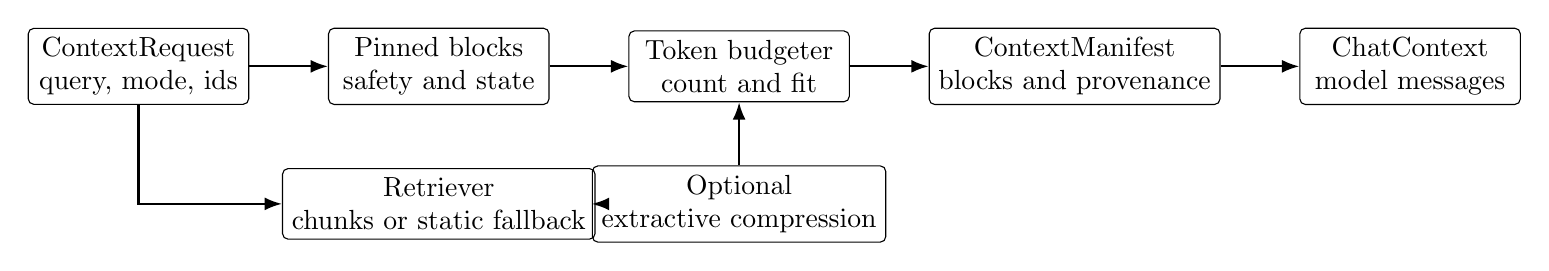
\begin{tikzpicture}[
  node distance=0.8cm and 1.0cm,
  box/.style={draw, rounded corners=2pt, align=center, minimum width=2.8cm, minimum height=0.8cm},
  arrow/.style={-{Latex[length=2.2mm]}, thick}
]
  \node[box] (request) {ContextRequest\\query, mode, ids};
  \node[box, right=of request] (pinned) {Pinned blocks\\safety and state};
  \node[box, below=of pinned] (retrieve) {Retriever\\chunks or static fallback};
  \node[box, right=of pinned] (budget) {Token budgeter\\count and fit};
  \node[box, below=of budget] (compress) {Optional\\extractive compression};
  \node[box, right=of budget] (manifest) {ContextManifest\\blocks and provenance};
  \node[box, right=of manifest] (chat) {ChatContext\\model messages};

  \draw[arrow] (request) -- (pinned);
  \draw[arrow] (request) |- (retrieve);
  \draw[arrow] (pinned) -- (budget);
  \draw[arrow] (retrieve) -- (compress);
  \draw[arrow] (compress) -- (budget);
  \draw[arrow] (budget) -- (manifest);
  \draw[arrow] (manifest) -- (chat);
\end{tikzpicture}
\end{center}

The manifest contains:

\begin{itemize}[leftmargin=*]
  \item \textbf{Blocks}: serialized model-facing context blocks.
  \item \textbf{Excluded patterns and blocked paths}: what was intentionally kept out.
  \item \textbf{Warnings}: approximate tokenization, truncation, non-authoritative memory, unavailable optional context, and similar conditions.
  \item \textbf{Budget report}: tokenizer name, active model profile, maximum input tokens, used input tokens, and approximate-token warnings.
  \item \textbf{Role summary}: counts of pinned, retrieved, and derived blocks.
  \item \textbf{Selected chunks}: references for query-aware retrieval.
  \item \textbf{Context provenance}: source and trust records used to audit what entered context.
  \item \textbf{Untrusted context warnings}: deduplicated authority warnings for downstream display and manifests.
\end{itemize}

\section{Core Data Types}

\subsection{ContextRequest}

\texttt{ContextRequest} is a dataclass in \texttt{context\_pack.py}. It captures the local information needed to select context for a turn:

\begin{lstlisting}[language=Python]
@dataclass(frozen=True)
class ContextRequest:
    project_root: Path
    query: str = ""
    mode: str | None = None
    model_profile: str | None = None
    session_id: str | None = None
    objective_id: str | None = None
    task_id: str | None = None
    run_id: str | None = None
    safety_boundaries: list[str] | None = None
\end{lstlisting}

This type is deliberately small. It does not contain executable actions, approval grants, backend handles, or provider credentials. It is only an input to local selection and serialization.

\subsection{ContextBlock}

\texttt{ContextBlock} is the unit that can be serialized into the chat context. Each block has a kind, title, sanitized content, optional source, token estimate, truncation flag, role, optional score, chunk ids, retrieval metadata, and optional provenance id.

The role is one of:

\begin{itemize}[leftmargin=*]
  \item \texttt{pinned}: safety, policy, request, and stable Harness domain context.
  \item \texttt{retrieved}: query-selected or static project context.
  \item \texttt{derived}: compressed or otherwise transformed context.
\end{itemize}

This role split is important because pinned context is treated as part of the operating boundary, while retrieved context is treated as potentially untrusted information selected for relevance.

\subsection{ContextManifest}

\texttt{ContextManifest} is the return value from \texttt{pack\_chat\_context}. It is the audit envelope for the model-facing context. Its \texttt{to\_payload()} method preserves legacy fields and adds newer versioned metadata such as \texttt{budget\_report}, \texttt{role\_summary}, \texttt{selected\_chunks}, \texttt{context\_provenance}, and \texttt{untrusted\_context\_warnings}.

\subsection{ContextProvenanceRecord}

\texttt{ContextProvenanceRecord} is defined in \texttt{models.py}. It records:

\begin{itemize}[leftmargin=*]
  \item \texttt{source\_kind}: user prompt, repository file, tool output, artifact, generated plan, memory record, task metadata, or run goal.
  \item \texttt{trust\_level}: trusted operator, untrusted repository, untrusted tool output, generated, artifact, or memory.
  \item \texttt{label}, \texttt{source\_id}, \texttt{artifact\_id}, \texttt{memory\_id}, and optional path.
  \item \texttt{sha256}, \texttt{redaction\_state}, lineage, and warnings.
\end{itemize}

The store builds run and task provenance in \texttt{SQLiteStore.build\_context\_provenance}. The context packer also creates provenance for blocks so that static, retrieved, memory, and artifact-derived content can be audited.

\section{Packing Flow}

\texttt{pack\_chat\_context} performs the following sequence.

\begin{enumerate}[leftmargin=*]
  \item Resolve the project root with \texttt{resolve\_project\_root}.
  \item Load context exclude patterns from config, falling back to \texttt{DEFAULT\_CONTEXT\_EXCLUDES}.
  \item Select a model profile and token budgeter.
  \item Build a \texttt{ContextRequest}.
  \item Add pinned candidates from \texttt{pack\_pinned\_context}.
  \item If the user turn has a non-empty query, retrieve dynamic chunks from the local chunk cache.
  \item If dynamic retrieval returns nothing, add static dynamic context from \texttt{pack\_static\_dynamic\_context}.
  \item Optionally compress eligible retrieved blocks when they exceed the remaining budget.
  \item Fit each block into the remaining token budget.
  \item Stop when the budget is exhausted or an oversized block is truncated.
  \item Build role summaries, selected chunk references, provenance, warnings, and the budget report.
\end{enumerate}

The key behavior is that retrieval is opportunistic. A query can select local chunks, but the system still has a deterministic static fallback that includes repository tree, README, AGENTS file, git status, diff summaries, recent artifact metadata, and compact operator context.

\section{Pinned Context}

Pinned context is built by \texttt{pack\_pinned\_context}. It includes:

\begin{longtable}{p{0.28\linewidth}p{0.62\linewidth}}
\toprule
\textbf{Block} & \textbf{Purpose} \\
\midrule
\texttt{harness\_vocabulary} & Defines Harness concepts such as objectives, tasks, leases, runs, adapters, isolated edits, apply-back, approvals, policy, and side-effect boundaries. \\
\texttt{builtin\_harness\_domain} & Serializes built-in workbenches, agents, model profiles, tool policies, and memory scopes from the registry. \\
\texttt{security\_policy\_summary} & Summarizes path guards, context excludes, hosted boundary requirements, adapter fail-closed behavior, and blocked-state codes. \\
\texttt{sandbox\_profiles} & Lists sandbox profile metadata. \\
\texttt{request\_context} & Includes current mode, model profile, session id, objective id, task id, run id, and safety boundaries when provided. \\
\texttt{memory\_summary} & Adds recent memory summaries with \texttt{memory\_not\_authority}; memory can inform but not authorize. \\
\bottomrule
\end{longtable}

Pinned context is not a permission source. For example, \texttt{request\_context} explicitly sets \texttt{permission\_granting: false}, and memory lineage includes \texttt{permission\_granting: false}, \texttt{policy\_authority: false}, and \texttt{approval\_authority: false}.

\section{Static Dynamic Context}

When query-aware retrieval does not provide chunks, the packer falls back to \texttt{pack\_static\_dynamic\_context}. These blocks describe the current project state:

\begin{itemize}[leftmargin=*]
  \item \texttt{repo\_tree}: up to \texttt{MAX\_TREE\_FILES} files, after excludes and secret-path filtering.
  \item \texttt{project\_file}: selected named files such as \texttt{README.md} and \texttt{AGENTS.md}, capped by \texttt{MAX\_FILE\_CHARS}.
  \item \texttt{git\_status}, \texttt{git\_diff\_stat}, and \texttt{git\_diff}: bounded git state.
  \item \texttt{recent\_artifacts}: artifact metadata only, not artifact bodies.
  \item \texttt{harness\_state}: compact operator context from \texttt{build\_operator\_context}.
\end{itemize}

Every file path is checked against configured context excludes. Secret-like paths are blocked through \texttt{assert\_not\_secret\_path}, and file contents are scanned with \texttt{scan\_text\_for\_secrets}. Binary and non-UTF-8 files are skipped with warnings.

\section{Token Budgeting}

\texttt{context\_budget.py} provides the budget abstraction:

\begin{lstlisting}[language=Python]
class TokenBudgeter(Protocol):
    name: str
    approximate: bool

    def count(self, text: str) -> int: ...
    def fit(self, text: str, max_tokens: int, *,
            marker: str = "\n[TRUNCATED: context budget]\n") -> TokenFit: ...
\end{lstlisting}

There are two implemented strategies.

\begin{itemize}[leftmargin=*]
  \item \texttt{HeuristicTokenBudgeter} uses the compatibility estimate \texttt{len(text) // 4}. It marks reports as approximate and emits \texttt{approximate\_token\_budget\_only}.
  \item \texttt{TiktokenBudgeter} is selected for OpenAI-like or Codex-like model profiles when \texttt{tiktoken} is installed. It uses \texttt{encoding\_for\_model} when possible and falls back to \texttt{cl100k\_base}.
\end{itemize}

\texttt{budgeter\_for\_project} chooses the budgeter from the active chat model profile. \texttt{legacy\_char\_budget\_to\_tokens} keeps the public \texttt{budget\_chars} API compatible while allowing token-aware internal fitting. \texttt{budget\_report} records the tokenizer, model profile, maximum input tokens, used input tokens, approximation state, and warnings.

The fitter uses a binary search over prefixes and preserves an explicit truncation marker. If the marker itself is too large, the largest marker prefix that fits is used. This keeps oversize context deterministic and bounded.

\section{Context Chunk Cache}

\texttt{context\_chunks.py} implements a persistent local cache of reusable context chunks. Chunks have the schema version \texttt{harness.context\_chunk/v1} and carry source, trust, path or source ids, line ranges, hash, size, token count, tokenizer, chunk scheme, sanitized text preview, redaction state, warnings, and metadata.

\subsection{Repository File Chunks}

\texttt{chunk\_repo\_file} splits UTF-8 repository files into line windows using the default scheme \texttt{line-v1:80}. It skips:

\begin{itemize}[leftmargin=*]
  \item context-excluded paths such as private Harness state, dependencies, caches, and build outputs,
  \item secret-like paths,
  \item binary files,
  \item files that cannot be decoded as UTF-8,
  \item text containing secret findings.
\end{itemize}

Repository chunks use \texttt{ContextSourceKind.REPO\_FILE} and \texttt{ContextTrustLevel.UNTRUSTED\_REPO}. Their metadata marks \texttt{permission\_granting: false}.

\subsection{Memory Chunks}

\texttt{chunk\_memory\_record} converts a memory summary into a context chunk. It uses \texttt{ContextSourceKind.MEMORY\_RECORD}, \texttt{ContextTrustLevel.MEMORY}, the scheme \texttt{memory-summary-v1}, and the warning \texttt{memory\_not\_authority}. It records memory scope, source kind, source artifact id, lineage, and explicit false authority flags.

Forgetting a memory record invalidates its chunks. Rebuilding memory chunks replaces changed summaries with new chunk ids because ids include the content hash.

\subsection{Artifact Metadata Chunks}

\texttt{chunk\_artifact\_metadata} indexes artifact metadata, not artifact bodies. It includes id, run id, session id, kind, path, hash, size, producer, redaction state, evidence status, sanitized metadata, and \texttt{contents\_included: false}. The warning \texttt{artifact\_body\_not\_indexed} makes this explicit.

\subsection{Persistence}

SQLite stores chunks in \texttt{context\_chunks}:

\begin{lstlisting}[language=SQL]
CREATE TABLE IF NOT EXISTS context_chunks (
  id TEXT PRIMARY KEY,
  schema_version TEXT NOT NULL,
  source_kind TEXT NOT NULL,
  trust_level TEXT NOT NULL,
  path TEXT,
  source_id TEXT,
  artifact_id TEXT,
  memory_id TEXT,
  start_line INTEGER,
  end_line INTEGER,
  sha256 TEXT NOT NULL,
  size_bytes INTEGER NOT NULL,
  token_count INTEGER,
  tokenizer TEXT,
  chunk_scheme TEXT NOT NULL,
  text_preview TEXT NOT NULL,
  redaction_state TEXT,
  warnings_json TEXT NOT NULL,
  metadata_json TEXT NOT NULL,
  created_at TEXT NOT NULL,
  updated_at TEXT NOT NULL
);
\end{lstlisting}

Indexes on \texttt{(source\_kind, path)} and \texttt{(sha256, chunk\_scheme, tokenizer)} support source lookup, stale cleanup, and idempotent rebuilds.

\section{Retrieval}

\subsection{Lexical Retrieval}

\texttt{context\_retrieval.py} implements \texttt{LexicalContextRetriever}. It reads cached chunks from SQLite and scores them against query terms.

The retriever:

\begin{itemize}[leftmargin=*]
  \item tokenizes query, preview text, paths, filenames, and symbols,
  \item boosts exact query matches in preview and path,
  \item boosts filename and path matches more than plain preview matches,
  \item downweights memory and generated/artifact sources,
  \item deduplicates equivalent chunks by source, path, line range, and hash,
  \item normalizes scores relative to the best selected result,
  \item returns manifest references with score, rank, retriever, trust metadata, hashes, line ranges, and warnings.
\end{itemize}

Retrievability checks mirror the chunking safety model. Missing files, excluded paths, secret-like paths, secret-containing previews, and invalid memory authority warnings are filtered out.

\subsection{Hybrid Local Retrieval}

\texttt{context\_vector.py} implements a local derived vector path. It uses \texttt{LocalHashEmbeddingProvider}, a deterministic 64-dimensional hashed bag-of-words embedder, and \texttt{LocalVectorIndex}. No hosted embedding provider is called.

The vector index stores \texttt{VectorRecord} rows with:

\begin{itemize}[leftmargin=*]
  \item vector id,
  \item chunk id,
  \item embedding provider id,
  \item dimension and quantization,
  \item source chunk hash,
  \item serialized vector,
  \item metadata containing source kind, trust level, path, memory id, artifact id, and authority flags.
\end{itemize}

SQLite stores vectors in \texttt{context\_vectors}, with a unique index on \texttt{(chunk\_id, embedding\_provider\_id)}. Health checks report missing chunks, stale vectors whose stored source hash no longer matches, and orphan vectors whose chunk is no longer indexable.

\texttt{HybridContextRetriever} combines lexical and dense local retrieval when dense retrieval is enabled. It uses reciprocal rank fusion and emits \texttt{hybrid\_rrf} results. If dense retrieval fails or has no hits, it falls back to lexical results.

\section{Compression}

\texttt{context\_compression.py} provides deterministic extractive compression through \texttt{ExtractiveContextCompressor}. It is intentionally conservative.

A block is eligible only when:

\begin{itemize}[leftmargin=*]
  \item its role is \texttt{retrieved},
  \item it has retrieval metadata,
  \item it is not a pinned or authority-sensitive block,
  \item it is not memory context,
  \item its source kind is \texttt{repo\_file}.
\end{itemize}

Compression selects lines around query-term matches and definition-like lines, removes simple boilerplate duplicates, preserves warning lines, adds the marker \texttt{[COMPRESSED: deterministic extractive context]}, and records lineage with the method, original and compressed token counts, original line count, selected lines, original chunk ids, provenance ids, and explicit false authority flags.

The compressor does not summarize policy, approvals, memory warnings, diffs, artifact metadata, or generated authority-related text. That is intentional: the implementation reduces retrieved code/file text while preserving source boundaries and avoiding invented authority.

\section{Context Transmission Policy}

\texttt{context\_policy.py} centralizes local-vs-hosted decisions.

\begin{longtable}{p{0.32\linewidth}p{0.18\linewidth}p{0.40\linewidth}}
\toprule
\textbf{Destination class} & \textbf{Default} & \textbf{Reason} \\
\midrule
\texttt{local\_process}, \texttt{local\_sqlite}, \texttt{local\_vector\_index} & Allowed & Local inspection and indexing are passive and do not grant execution authority. \\
\texttt{hosted\_embedding}, \texttt{hosted\_reranker}, \texttt{hosted\_model}, \texttt{hosted\_compression} & Denied & Hosted transmission needs a future explicit approval path. \\
\texttt{remote\_vector\_store}, \texttt{pgvector}, \texttt{qdrant}, \texttt{weaviate}, \texttt{milvus} & Denied & Remote vector stores are unsupported in this release and fail closed. \\
Unknown destination & Denied & Unknown context destinations fail closed. \\
\bottomrule
\end{longtable}

Any secret-like, excluded, or forgotten context is denied for every destination. Policy decisions also propagate warnings such as \texttt{memory\_not\_authority} and \texttt{untrusted\_context}. Decision payloads explicitly state that no provider call, Docker permission, adapter dispatch, approval authority, policy authority, or active repository mutation is granted.

\section{Chat Integration}

\texttt{chat.py} uses the context pipeline in the normal model turn path. \texttt{\_model\_chat\_response} builds:

\begin{enumerate}[leftmargin=*]
  \item the operator-facing context payload via \texttt{chat\_context(project\_root)},
  \item the packed manifest via \texttt{pack\_chat\_context(project\_root, query=raw, mode=mode, model\_profile=model\_profile, safety\_boundaries=...)},
  \item progress lines for selected context blocks,
  \item a \texttt{ChatContext} containing serialized manifest blocks and safety boundaries,
  \item model messages through \texttt{\_model\_messages}.
\end{enumerate}

After the model turn, the read-only tool loop can fetch more detail through controlled tools such as repository tree, file reads, search, diff, and JSON context tools. If the model asks for an action contract or an unknown tool, the chat layer routes through the existing action-contract and rejection paths. Context packing itself does not perform those actions.

The autonomous read loop also constructs a \texttt{ChatContext} from \texttt{pack\_chat\_context}, but action execution remains governed by autonomy policy and Harness validation.

\section{CLI and API Surfaces}

The CLI exposes context inspection and maintenance commands in \texttt{src/harness/cli/main.py}.

\begin{longtable}{p{0.30\linewidth}p{0.60\linewidth}}
\toprule
\textbf{Command} & \textbf{Behavior} \\
\midrule
\texttt{harness context inspect} & Packs context and prints or emits the manifest without executing providers or tools. \\
\texttt{harness context estimate} & Estimates packed context token use and emits the budget report. \\
\texttt{harness context chunks} & Lists cached context chunks without rebuilding. \\
\texttt{harness context search} & Runs local lexical retrieval over cached chunks. \\
\texttt{harness context policy} & Explains the fail-closed transmission decision for a destination. \\
\texttt{harness context rebuild-chunks} & Explicitly rebuilds repo, memory, and artifact metadata chunks. This writes local SQLite state. \\
\texttt{harness context rebuild-index} & Explicitly rebuilds the derived local vector index. This writes local SQLite vector rows. \\
\bottomrule
\end{longtable}

The local server exposes \texttt{/sessions/\{session\_id\}/context/estimate}. This route estimates composer context budget from prompt text, mentions, attachments, and optional instruction-file metadata without loading referenced file contents. The response includes \texttt{contents\_included: false}, \texttt{permission\_granting: false}, and \texttt{execution\_started: false}. The estimate is persisted as a redacted \texttt{session.context.estimated} event.

\section{Safety Invariants}

The implementation repeatedly enforces the same invariants across packers, chunkers, retrievers, vector indexing, CLI, and API routes.

\begin{enumerate}[leftmargin=*]
  \item \textbf{Context is passive.} Context inspection does not start providers, Docker, adapters, or mutation workflows.
  \item \textbf{Excluded state stays excluded.} \texttt{.harness}, \texttt{.git}, dependency folders, build outputs, and configured excludes are omitted from normal context.
  \item \textbf{Secret-like content is blocked.} Secret-like paths and text findings are not packed, chunked, retrieved, or indexed.
  \item \textbf{Artifacts are metadata-first.} Recent artifact context and artifact chunks avoid artifact bodies unless a separate explicit projection is designed to include a bounded preview.
  \item \textbf{Memory is non-authoritative.} Memory is useful context, but it always carries \texttt{memory\_not\_authority} and false authority flags.
  \item \textbf{Repository text is untrusted.} Repository file chunks and provenance use \texttt{untrusted\_repo}; retrieved repo text cannot override Harness policy.
  \item \textbf{Hosted transmission fails closed.} Hosted and remote context destinations are denied by default.
  \item \textbf{Budget overflow is visible.} Truncation and compression add markers and warnings rather than silently dropping context.
\end{enumerate}

\section{Test Coverage}

The context implementation is covered by focused unit and integration tests.

\begin{longtable}{p{0.34\linewidth}p{0.56\linewidth}}
\toprule
\textbf{Test file} & \textbf{Coverage} \\
\midrule
\texttt{tests/test\_context\_budget.py} & Token counting, fitting, tokenizer fallback, budget reports, and approximation warnings. \\
\texttt{tests/test\_context\_pack.py} & Static packing, pinned roles, dynamic roles, excludes, secret blocking, artifact metadata exclusion, memory warnings, request context, budget truncation, provenance, and untrusted warnings. \\
\texttt{tests/test\_context\_chunks.py} & Chunk schema round trips, repo chunk filtering, idempotent rebuilds, stale replacement, memory chunk invalidation, and artifact metadata-only chunks. \\
\texttt{tests/test\_context\_retrieval.py} & Local lexical search behavior, filtering, ranking, deduplication, and manifest references. \\
\texttt{tests/test\_context\_vector.py} & Local vector rebuilds, health checks, stale/orphan cleanup, memory invalidation, lexical fallback, and hybrid retrieval. \\
\texttt{tests/test\_context\_compression.py} & Extractive compression eligibility, deterministic output, preserved warnings, line selection, and budget fitting. \\
\texttt{tests/test\_context\_policy.py} & Local allow decisions, hosted and remote denial, secret/excluded denial, and warning aggregation. \\
\texttt{tests/test\_local\_server.py} & Session context estimate API, metadata-only behavior, event persistence, and absence of referenced file bodies from estimate responses. \\
\texttt{tests/test\_cli\_smoke.py} & CLI chat context behavior, JSON context output, TUI context surfaces, context estimates, provenance, and warning propagation. \\
\bottomrule
\end{longtable}

\section{Why the Implementation Uses a Manifest}

The manifest is the stabilizing abstraction. Without it, the chat layer would only know that it had a blob of text. With it, Harness can answer:

\begin{itemize}[leftmargin=*]
  \item Which blocks were pinned versus retrieved?
  \item Which chunks were selected and why?
  \item Which paths were blocked?
  \item Which tokenizer and model profile were used for estimates?
  \item Was any block truncated or compressed?
  \item Did any context come from memory, generated text, artifacts, tool output, or untrusted repository files?
  \item Which warnings should be shown to the operator or included in run manifests?
\end{itemize}

This is why context is represented as structured data first and serialized into model messages only at the boundary where the backend needs messages.

\section{Current Limitations}

The implemented system is intentionally conservative.

\begin{itemize}[leftmargin=*]
  \item The dense index is a local hashed bag-of-words index, not a semantic hosted embedding system.
  \item Hosted embeddings, rerankers, remote vector stores, and hosted compression are denied.
  \item Artifact chunks index metadata only, not full artifact contents.
  \item Compression is extractive and deterministic; it does not perform abstractive summarization.
  \item Static fallback context can still be coarse when no chunk cache has been rebuilt.
  \item The legacy \texttt{budget\_chars} parameter remains for compatibility, although internal fitting is token-oriented.
\end{itemize}

These limitations are aligned with the release goal: improve relevance and auditability without weakening the local-first authority boundary.

\section{Summary}

Harness context is implemented as a local, structured, auditable pipeline. Pinned blocks preserve the operating boundary; retrieved blocks improve relevance; chunk and vector caches make retrieval repeatable; token budgeting bounds model input; compression reduces oversized retrieved file text without inventing content; provenance and warnings preserve authority information; and policy decisions prevent accidental hosted or remote transmission. The result is a context system that gives the model useful project information while keeping Harness, not the model context, responsible for permissions, approvals, policy, and side effects.

\end{document}
